\chapter{System Design and Architecture}
\label{Chapter2}

This chapter presents the design and architecture of our constrained procedural terrain generation system. Building upon the limitations of existing approaches identified in Chapter \ref{Chapter1}, we develop a modular system that addresses the key challenges through a \textbf{distance-based} methodology.

We first establish our system requirements and design objectives, then detail the component-based architecture that enables flexible combinations of terrain operations. We explain our overall workflow and conclude with Unity-specific implementation considerations. The mathematical foundations of our distance-based approach are detailed in Chapter \ref{Chapter3}, while the Interactive Genetic Algorithm for parameter optimisation is covered in Chapter \ref{Chapter4}.

\section{System Requirements and Design Goals}

In response to the challenges discussed in previous sections, we established the following system requirements and design goals to guide the development of our terrain generation framework.

\subsubsection{Core Requirements}

\begin{itemize}
    \item \textbf{Constraint Preservation}: Fixed points must maintain their exact heights throughout the generation process -- we never modify the heights of these areas. We use \textbf{mask} \textbf{textures} where red pixels indicate fixed areas and black pixels represent modifiable regions. This intuitive format integrates well with standard image editing tools (see Figure \ref{fig:mask_examples});

    \item \textbf{Natural Transitions}: The system should create \textit{smooth, realistic transitions} between fixed and generated terrain, avoiding the abrupt discontinuities that typically occur when applying traditional procedural techniques to constrained problems; 

    \item \textbf{Algorithmic Flexibility}: The architecture should accommodate \textit{a variety} of terrain generation techniques without requiring algorithm-specific modifications for constraint handling. This enables integration of Perlin noise, Voronoi Diagrams, and Midpoint Displacement methods.
    
\end{itemize}

\subsubsection{Design Objectives}

Based on these requirements, we defined the following five key objectives:

\begin{itemize}
    \item \textbf{Modular Architecture}: Enable flexible combinations of terrain operations using a component-based design that cleanly separates responsibilities;
    
    \item \textbf{Distance-Based Processing}: Use proximity to fixed points to guide terrain modifications;
    
    \item \textbf{Intuitive Parameter Tuning}: Provide both manual control and automated parameter exploration through Interactive Genetic Algorithms;
    
    \item \textbf{Performance Optimisation}: Leverage GPU acceleration for computationally intensive operations;
    
    \item \textbf{Extensibility}: Allow easy addition of new terrain operations and constraint types.
\end{itemize}

These objectives ensure our system serves both novice users seeking accessible terrain generation and expert users requiring precise control.

\subsubsection{Architectural Approach}
\label{top_down_approach}

We adopt a \textbf{top-down approach}, in which we first generate the entire terrain using traditional methods, and then adjust it to respect the given constraints. Specifically, in the modifiable areas (represented by black pixels in the mask), we initially run the procedural terrain generation algorithms without considering the constraints. This is illustrated in Figure \ref{fig:top_down_example}, where the constrained regions remain untouched and do not yet influence the surrounding terrain. 


\begin{figure}[h!]
    \centering
    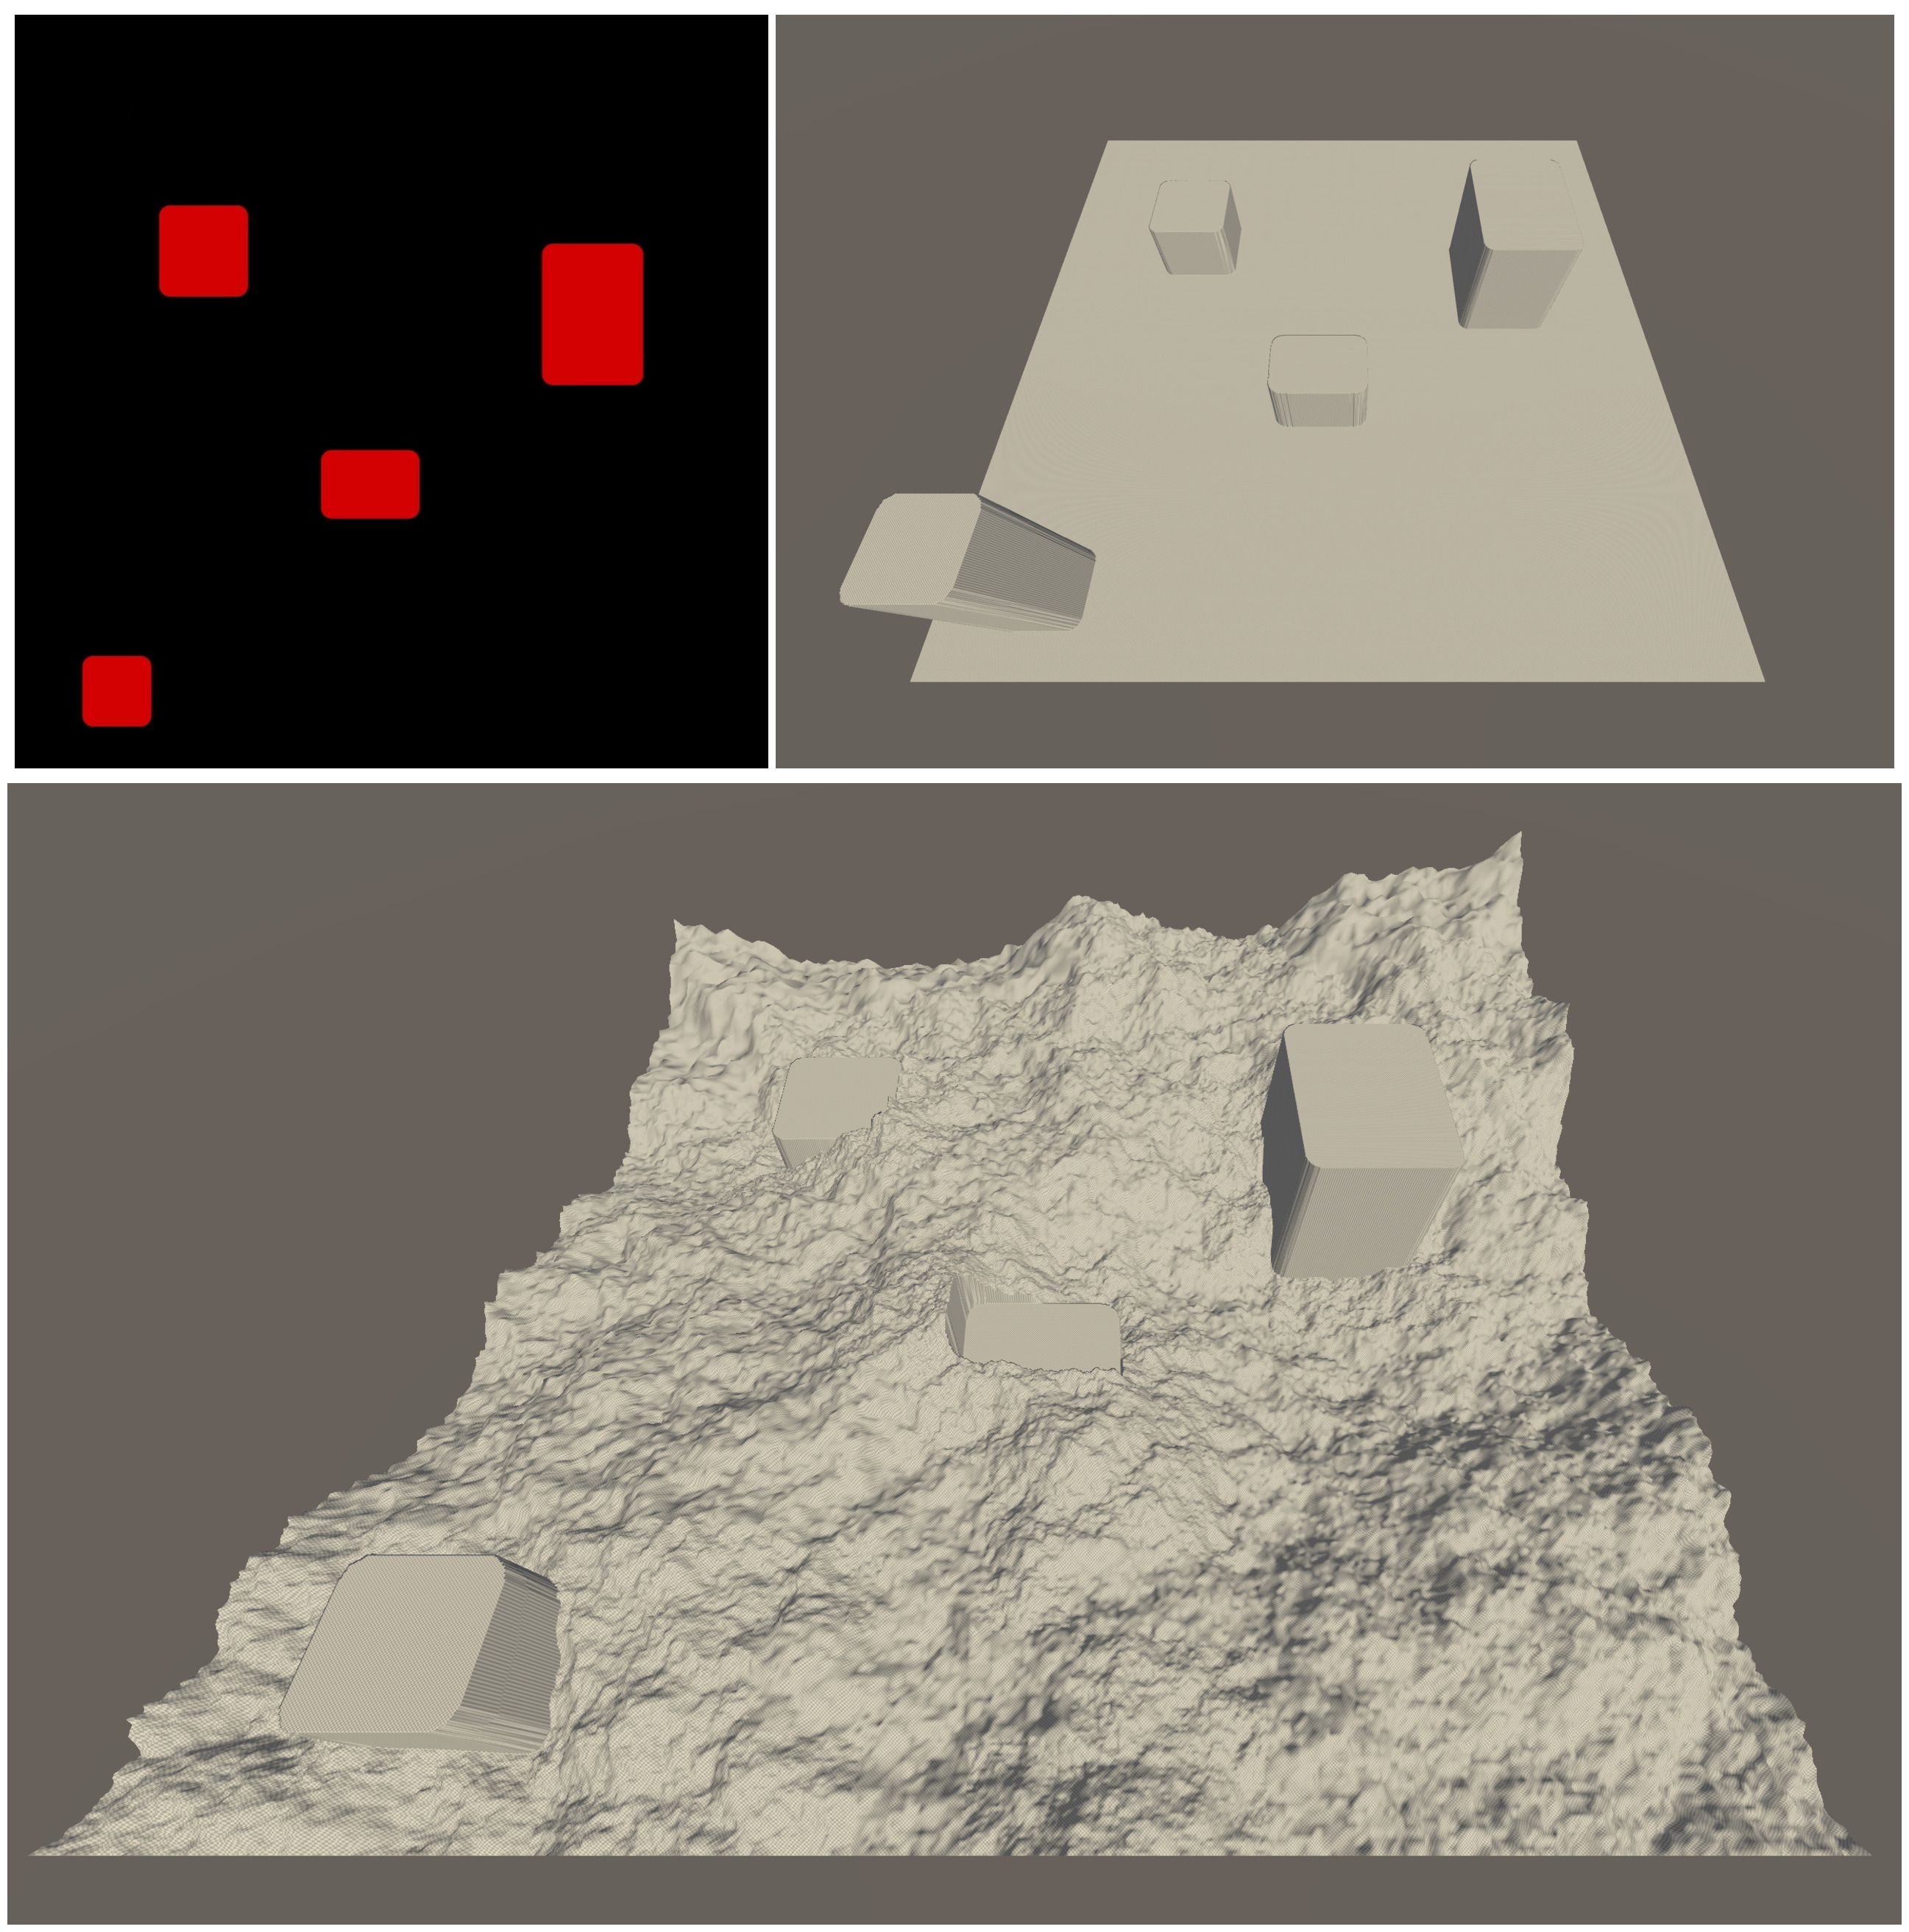
\includegraphics[width=0.7\linewidth]{img/Chapter_2_images/building_example_top_down.jpg}
    \caption{\textbf{Top left} Shows the mask texture, with red pixels indicating constrained areas, and black pixels indicating modifiable areas; \textbf{top right} shows the predefined heights of the constrained areas in the terrain, and all the modifiable pixels heights are currently set to 0; \textbf{bottom figure} shows resulting terrain after running midpoint displacement algorithm, before applying any post-processing to smooth out transitions.}

    \label{fig:top_down_example}
\end{figure}

In the second step, we apply \textbf{post-processing} to modify the surrounding terrain so that it blends smoothly into the constrained areas (identified by red pixels in the mask).

This contrasts with the \textbf{bottom-up} methods that propagate constraints outward from fixed points using \textit{Inverse Midpoint Displacement} \citep{Belhadj07}. Our approach offers greater flexibility and compatibility with existing algorithms, requiring only that operations respect the constraint mask, rather than implementing specialised \textit{constraint-aware} algorithms.

This architectural decision profoundly influences our system design, enabling the modular, component-based structure that separates constraint handling from specific terrain generation techniques.

\section{Component-Based Architecture}
In this section we describe the actual component-based architecture of our system. We can see a visual representation of this structure in the diagram in Figure \ref{fig:component_diagram} below.

\begin{figure}[h!]
    \centering
    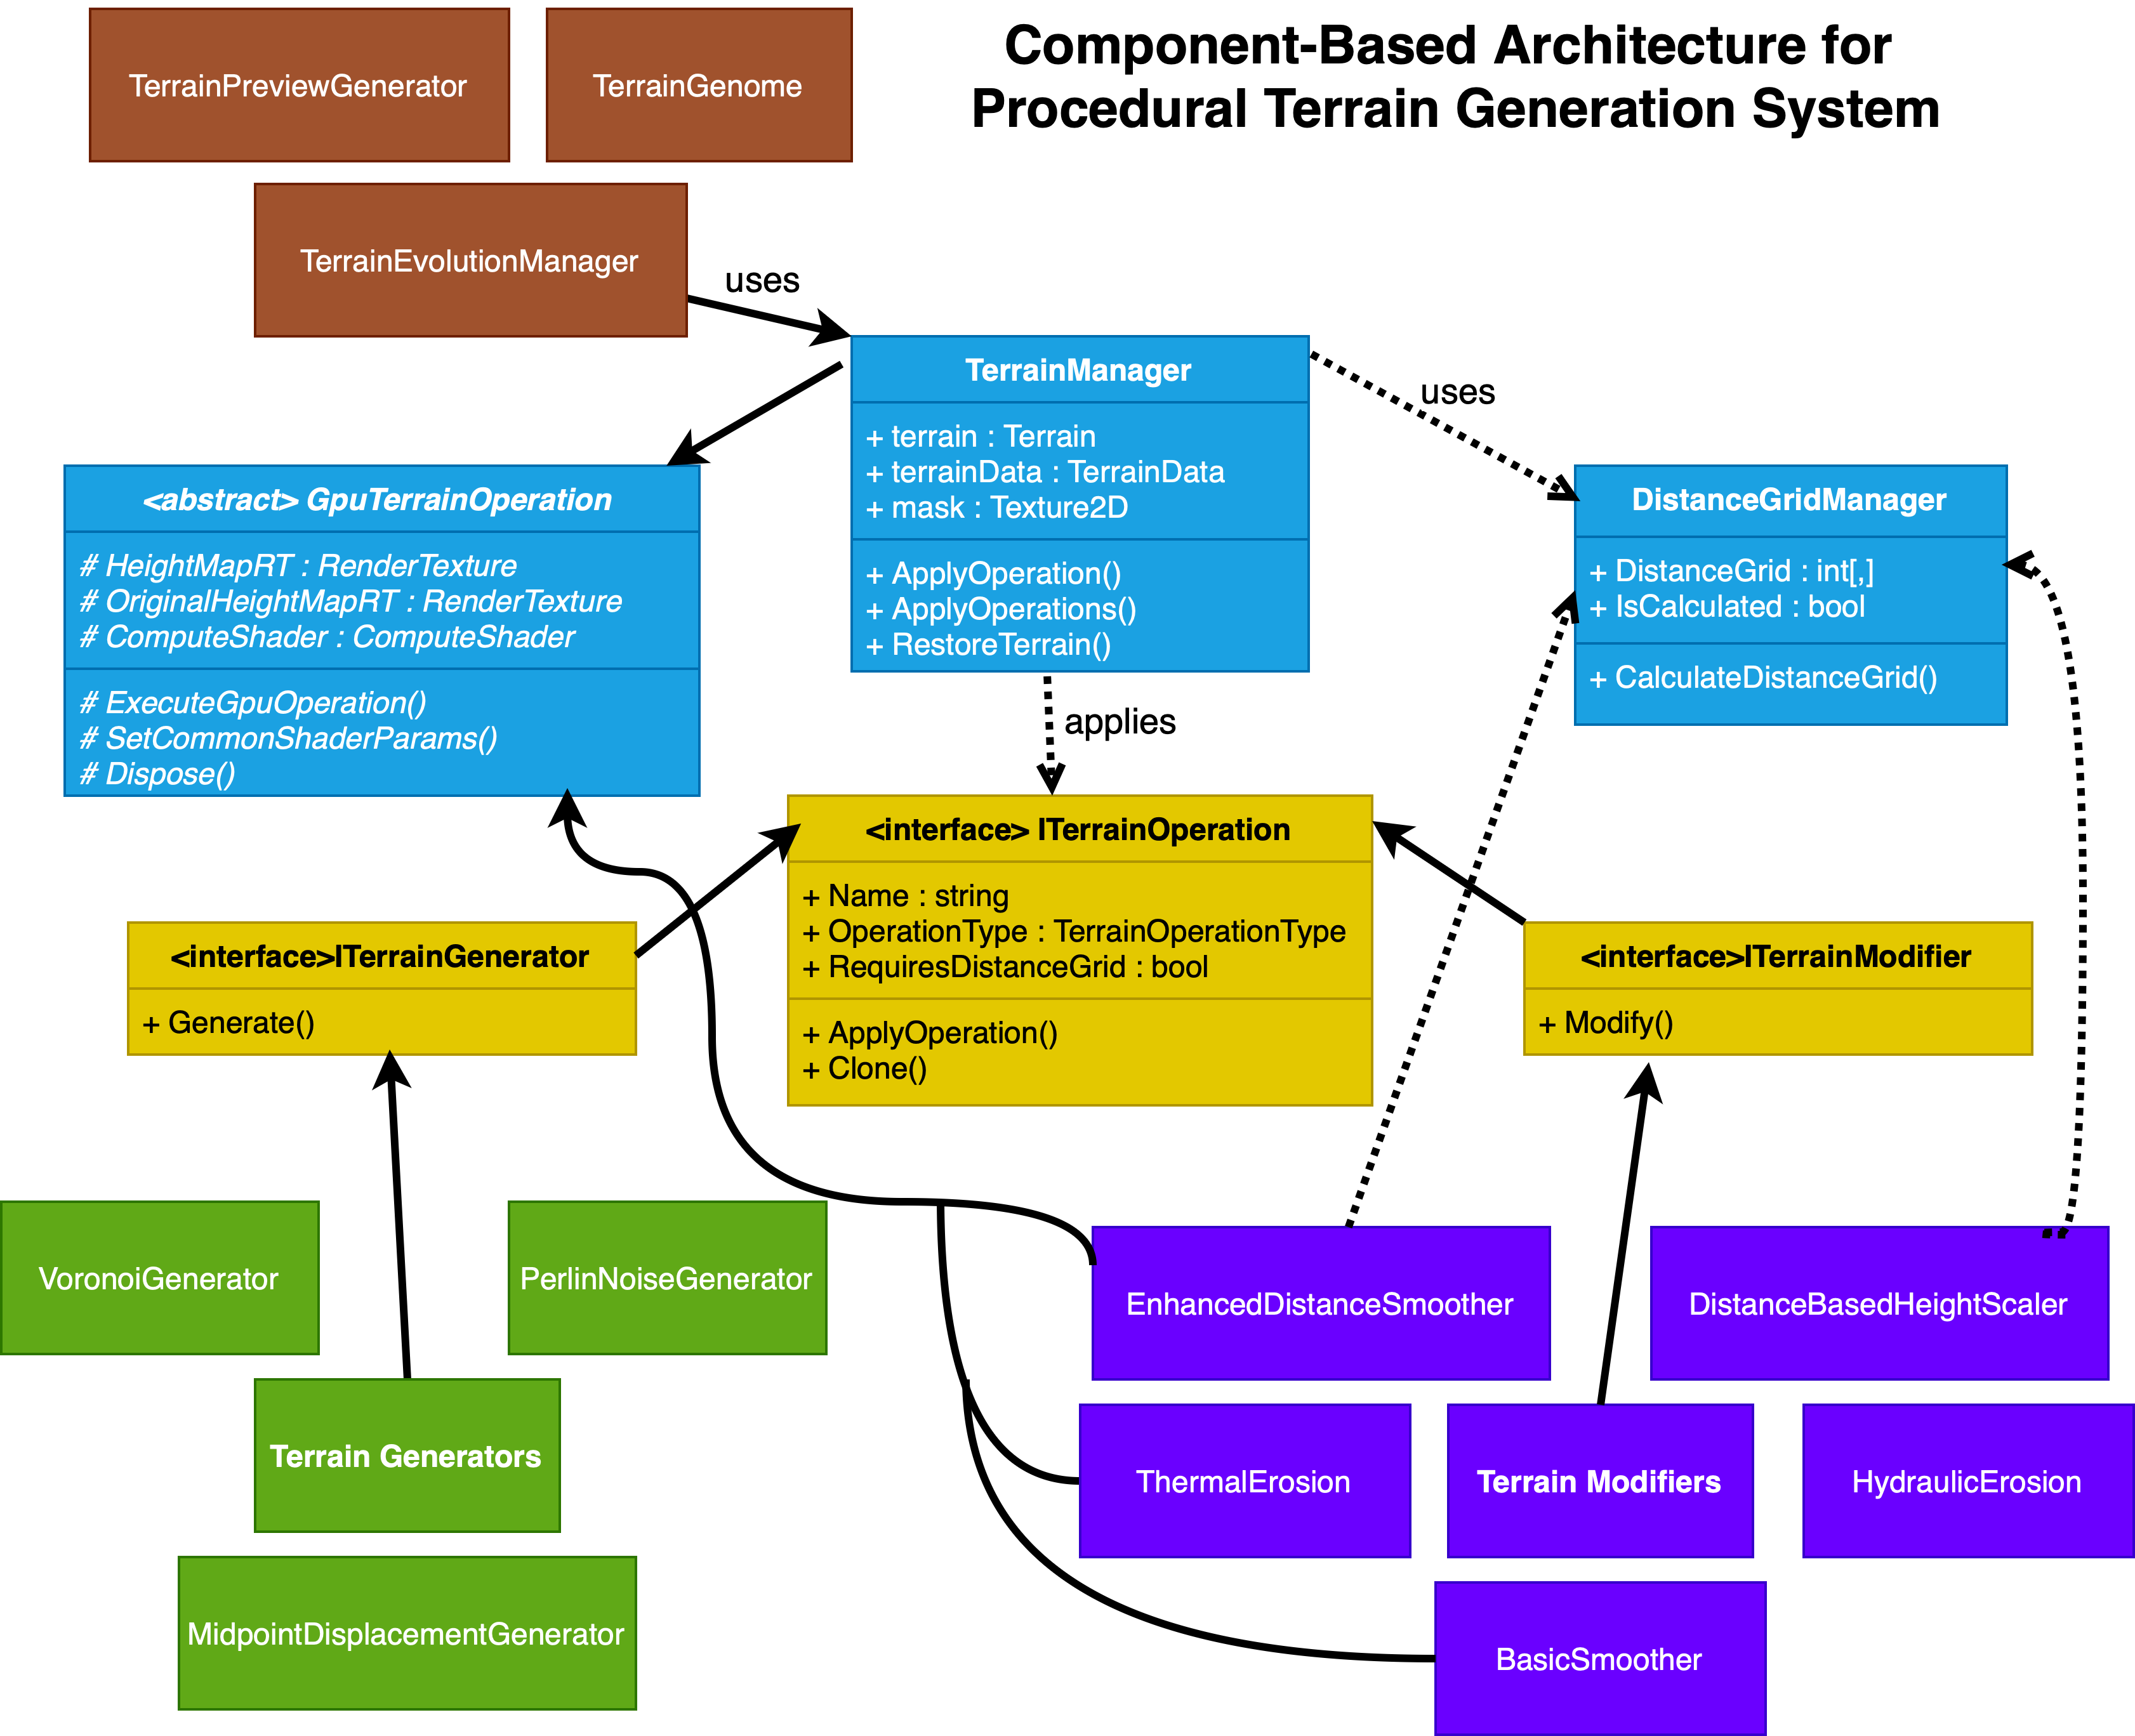
\includegraphics[width=1.0\textwidth]{img/Chapter_2_images/Diagrams/component_diagram.png}
    \caption{High-level architecture showing core components and relationships. The \textsf{TerrainManager} coordinates operations, while \textsf{ITerrainOperation} implementations provide specific algorithms to change the heights of modifiable areas in the terrain. \textsf{DistanceGridManager} supplies proximity information for distance-aware operations. \textsf{TerrainEvolutionManager} is how the IGA connects to the system. }
    \label{fig:component_diagram}
\end{figure}

% \subsection{Core Components}
Specifically, each component does the following:

\textbf{\textsf{TerrainManager}}: The central coordinator that manages Unity terrain objects, interprets constraint masks, and applies operations while preserving fixed heights. This component serves as the \textbf{primary interface} for both manual operation and IGA-based approaches.
    

\textbf{\textsf{ITerrainOperation} Interface}: All terrain operations implement this foundational interface, which defines the essential \textit{contract} for terrain modification. The interface specifies operation methods, distance grid requirements, and support for genetic algorithm operations through cloning.

Operations are categorised as either \textsf{ITerrainGenerator} (create terrain features) or \textsf{ITerrainModifier} (adjust existing terrain). This distinction aids organisation and user interface design, though both types follow the same operational pattern.
    
\textbf{\textsf{DistanceGridManager}}: Calculates and maintains distance information from each terrain point to the nearest fixed point using an efficient breadth-first search algorithm. This component enables distance-aware operations, forming a crucial part of our distance-based methodology (see Chapter \ref{Chapter3}).


\textbf{\textsf{GpuTerrainOperation}}: Base class for GPU-accelerated operations, handling compute shader management and CPU/GPU data transfer. This component provides automatic fallback to CPU implementations when GPU acceleration is unavailable. Technical implementation details are available in our system's source code.

\subsubsection{Operation Pipeline}

Our system applies operations \textbf{sequentially}, with each additional operation building upon the results of previous one. This pipeline approach enables:
\begin{itemize}
    \item Explicit control over operation ordering;
    \item Independent parameter adjustment for each operation;
    \item Easy experimentation with different operation combinations;
    \item Natural integration with genetic algorithm mutations and crossover.
\end{itemize}

The pipeline accommodates the full range of terrain operations available in our system. Complete parameter descriptions are available in the user documentation, while implementation specifics can be found in the source code.

\subsubsection{User Interaction Models}
\label{interaction_models}

Our architecture supports two distinct interaction approaches that serve different user needs and expertise levels:


\begin{itemize}
    \item \textbf{Manual Operation Approach}: Users directly select and configure terrain operations through Unity's inspector interface. This approach provides:
\begin{itemize}
    \item[-] Precise control over individual operation parameters;
    \item[-] Direct manipulation of operation sequences;
    \item[-] Immediate visual feedback for iterative refinement;
    \item[-] Full access to the complete parameter space for expert users.
\end{itemize}

This method suits users with terrain generation expertise who require fine-grained control over the generation process.

    
    \item \textbf{Interactive Genetic Algorithm Approach}:
The system generates populations of terrain variants with different operation sequences and parameters, allowing users to guide evolution through visual selection rather than manual parameter tuning. This approach, based on the pioneering work by \textcite{Walsh10}, enables:
\begin{itemize}
    \item[-] Intuitive exploration of complex parameter combinations;
    \item[-] Discovery of aesthetically pleasing solutions without technical expertise;
    \item[-] Guided evolution through user aesthetic preferences;
    \item[-] Accessible terrain generation for non-expert users\footnote{The complete IGA implementation and methodology are detailed in Chapter \ref{Chapter4}.}.
\end{itemize}

\end{itemize}

\section{Workflow Overview}

\begin{figure}[h!]
    \centering
    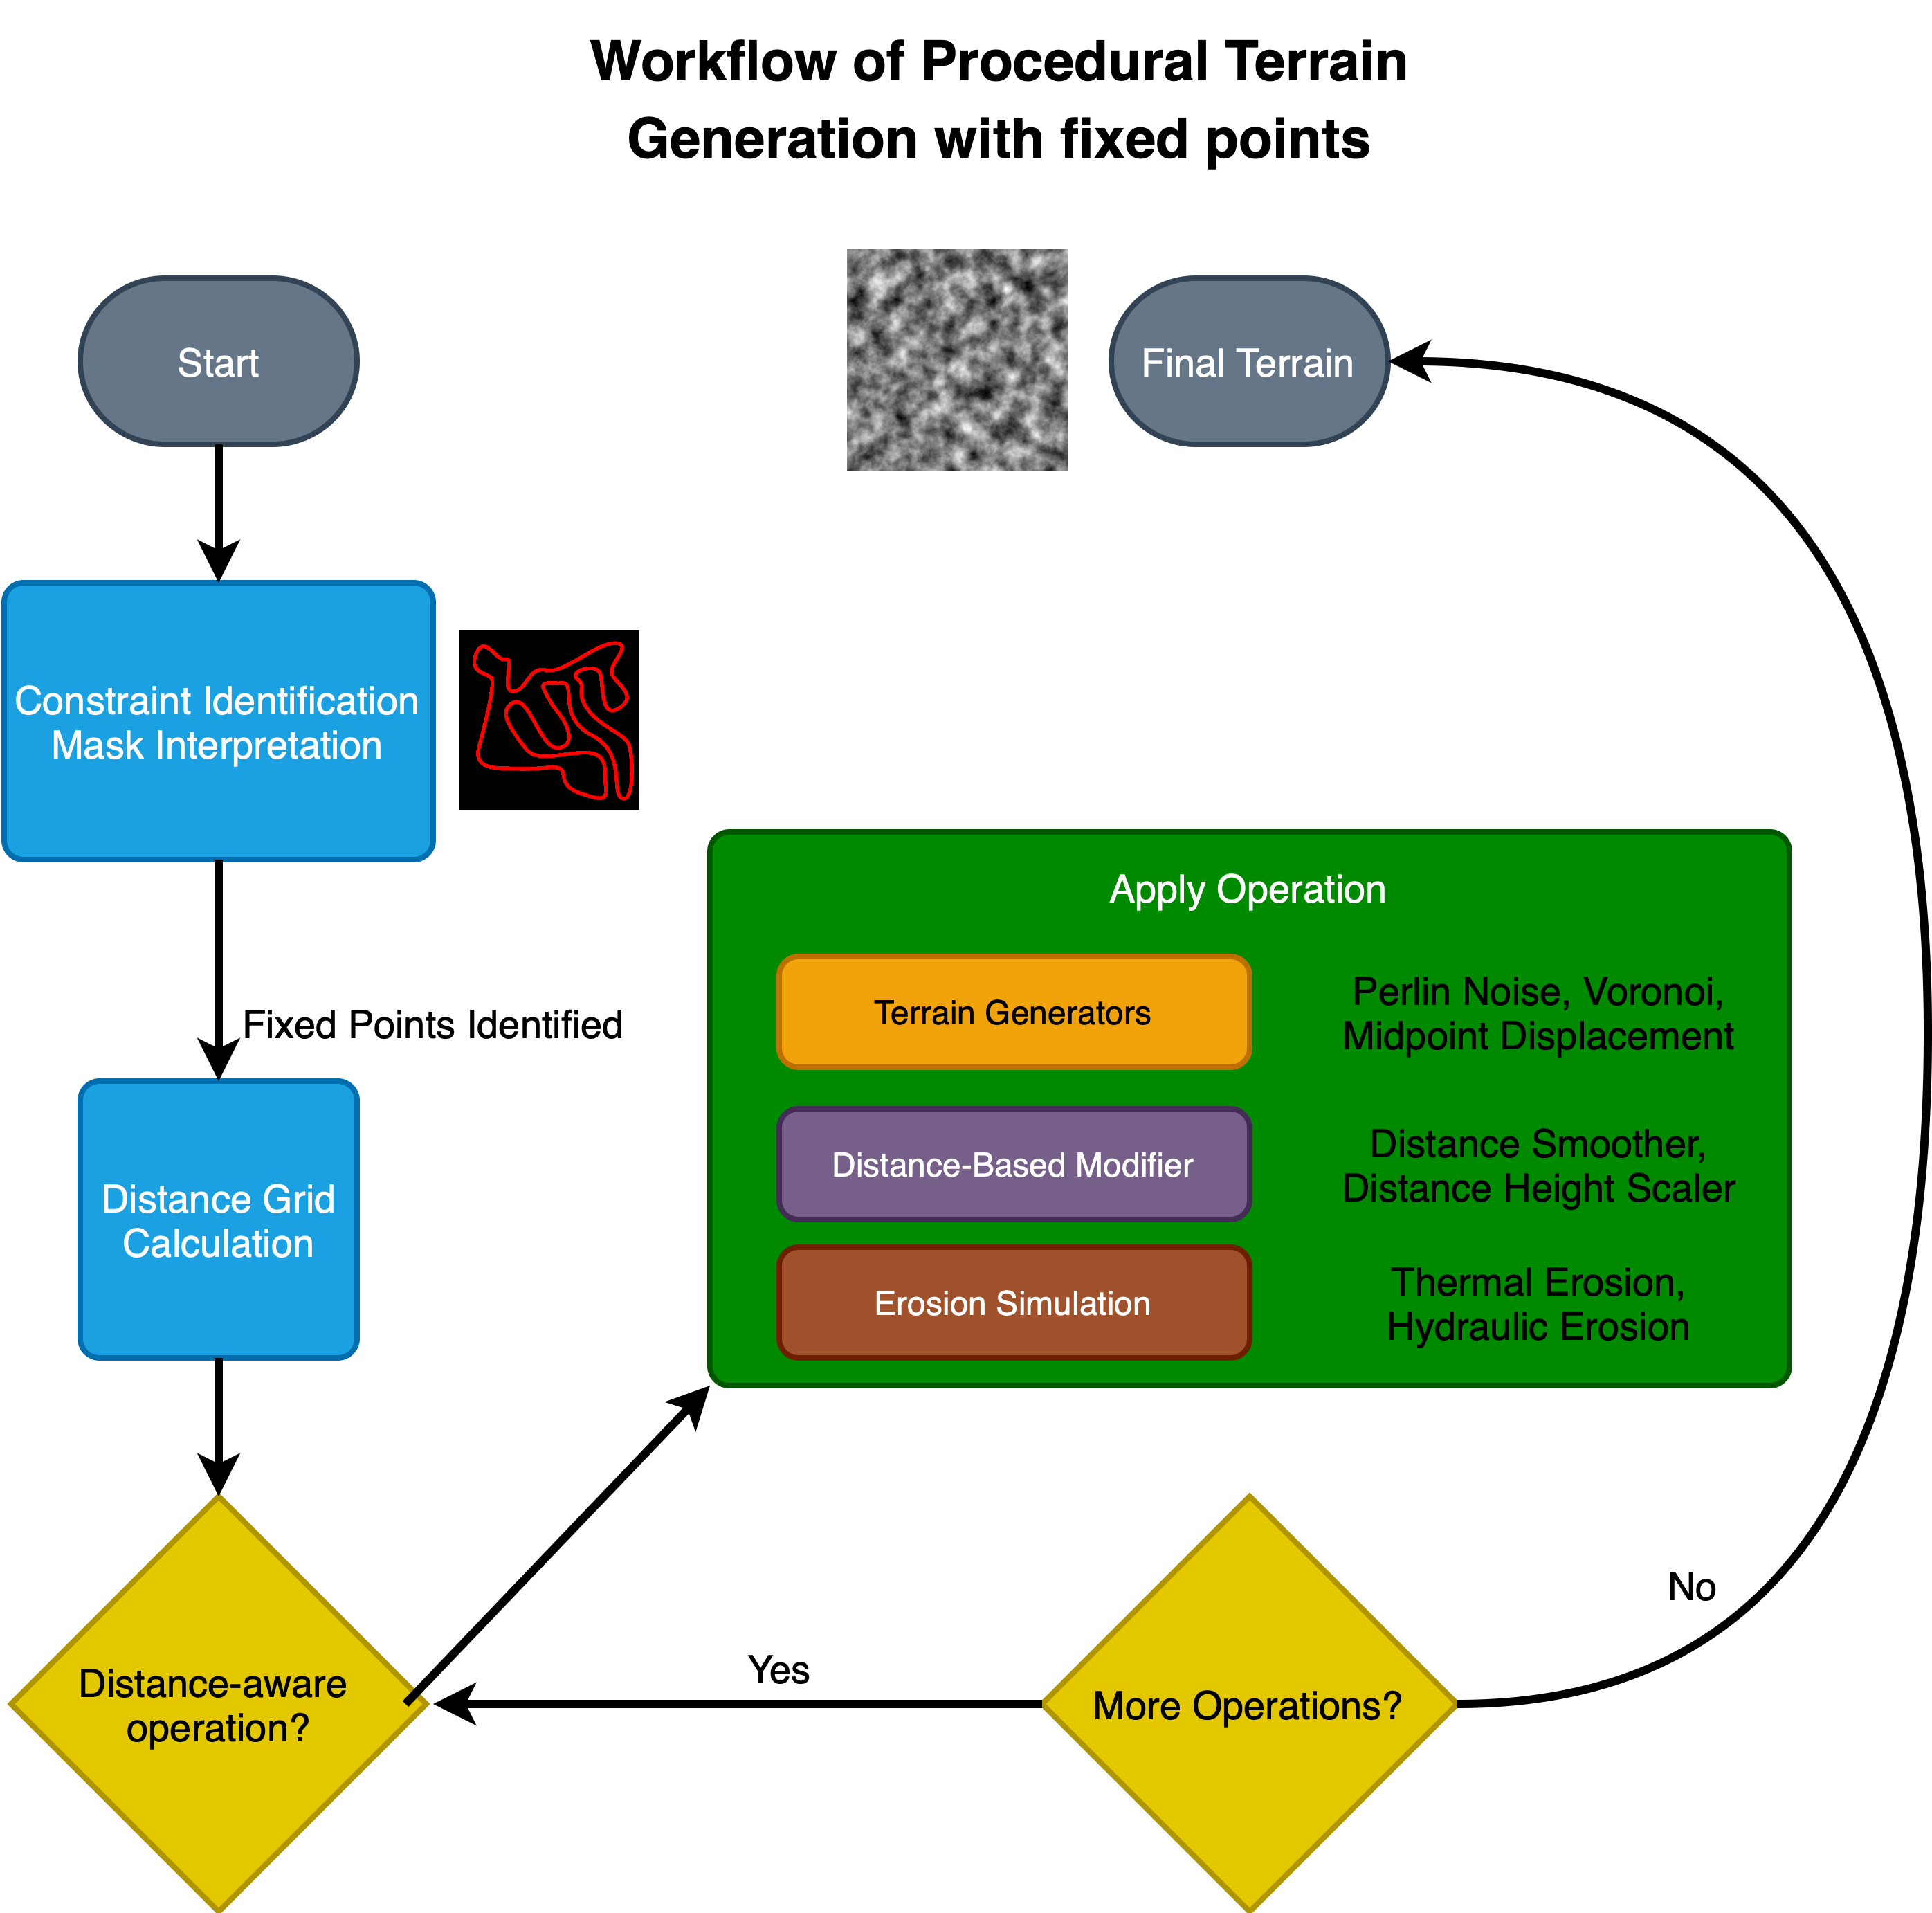
\includegraphics[width=1.0\textwidth]{img/Chapter_2_images/Diagrams/workflow_diagram.png}
    \caption{System workflow from constraint identification through terrain generation and modification. Distance grid calculation enables distance-aware operations to create natural transitions between fixed and generated areas.}
    \label{fig:workflow_diagram}
\end{figure}

Our system follows a five-stage workflow that transforms initial constraints into natural-looking terrain. A visual representation of this workflow can be seen in Figure \ref{fig:workflow_diagram}. This workflow is exactly the same whether users employ manual operation selection or the Interactive Genetic Algorithm approach.

\subsubsection{Constraint Identification}
\label{mask_interpretation}

The workflow begins with identifying fixed areas through mask textures. As we mentioned above, red pixels represent immutable heights, while black pixels indicate modifiable regions. 

\begin{figure}[h!]
    \centering
    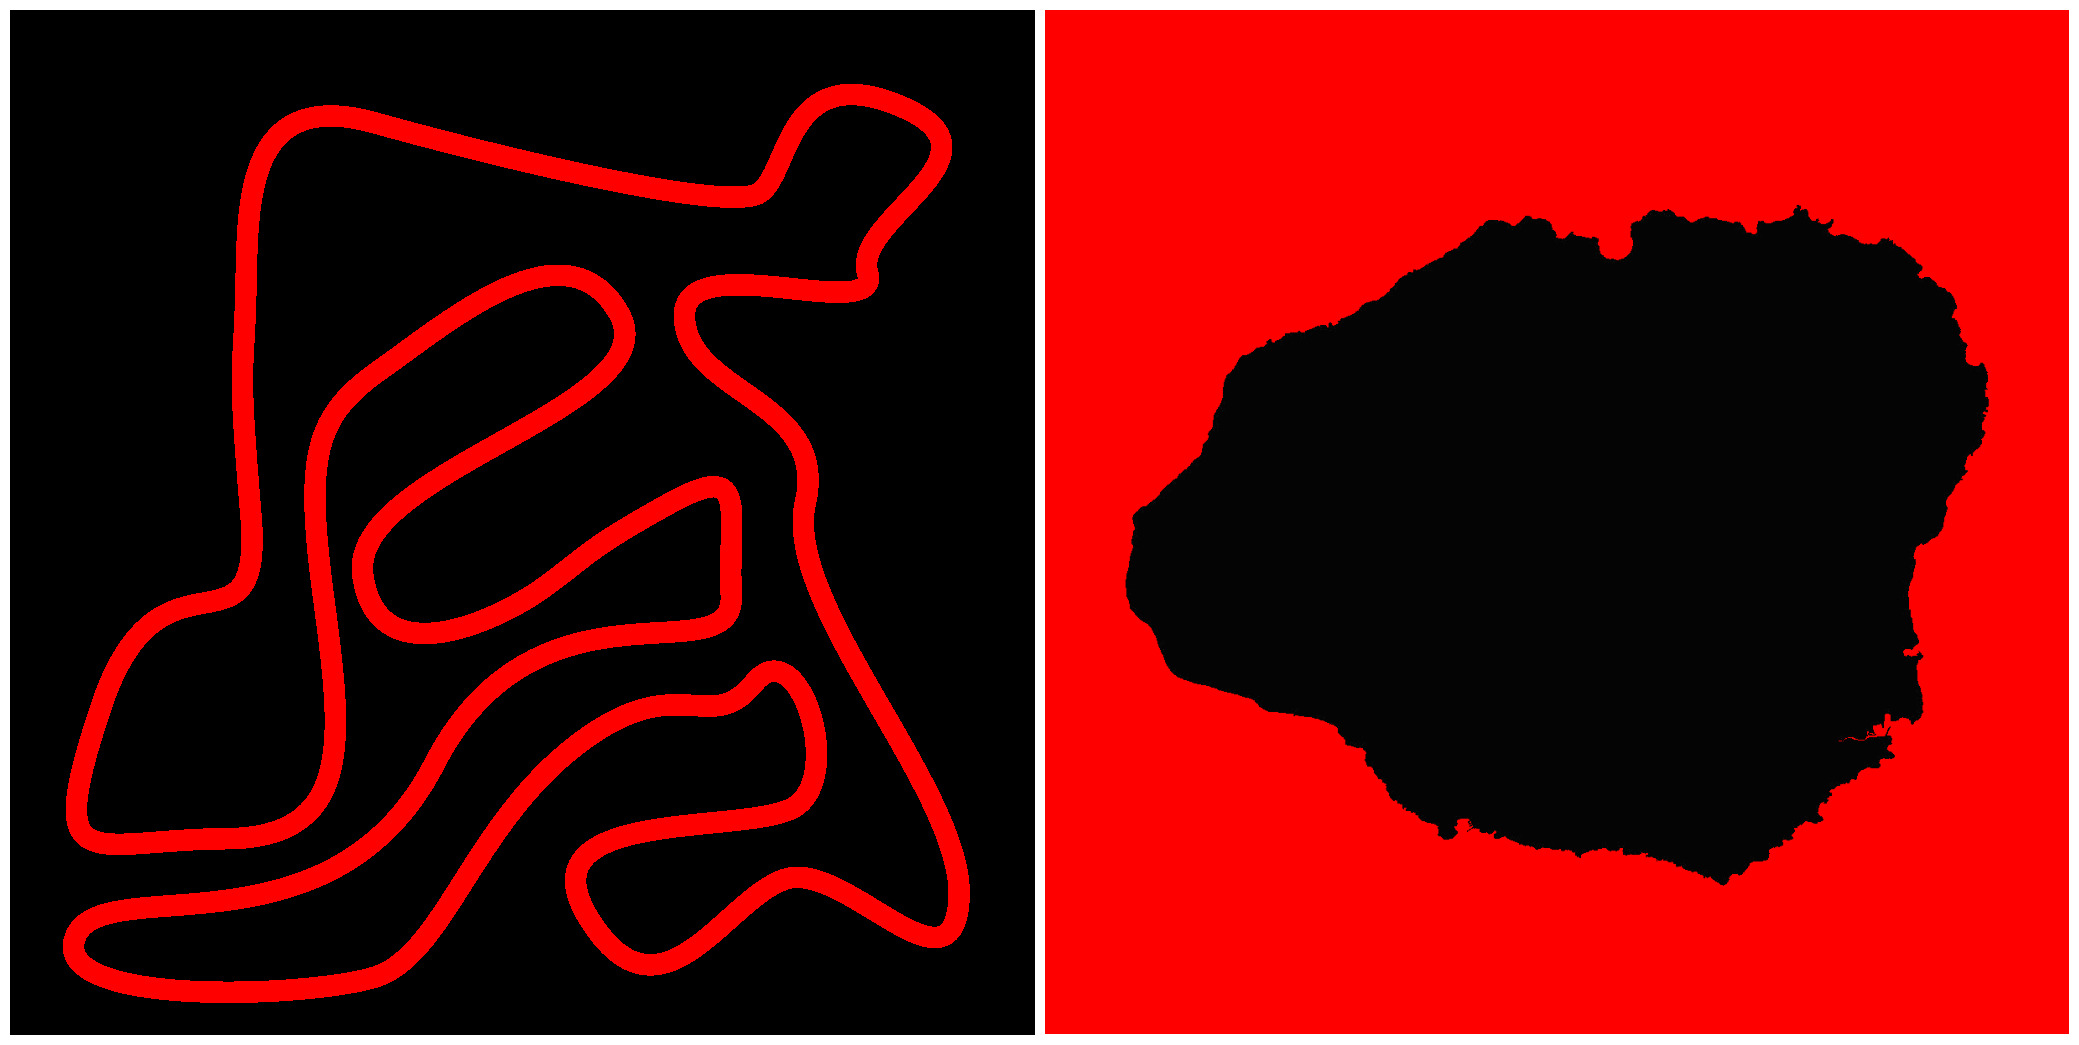
\includegraphics[width=0.8\textwidth]{img/Masks/mask_example.jpg}
    \caption{Example constraint masks representing different scenarios: racing track layout (left) where roads maintain fixed heights, and island coastline (right) where water levels remain constant. Red areas preserve exact heights while black areas allow procedural modification.}
    \label{fig:mask_examples}
\end{figure}

The mask interpretation system handles arbitrary constraint patterns, from simple geometric shapes to complex networks. This flexibility enables applications ranging from road integration to architectural site planning.

\subsubsection{Distance Grid Calculation}

For operations requiring distance information, the system calculates the minimum distance from each terrain point to the nearest fixed point. This distance grid enables adaptive terrain modifications that create natural transitions by varying operation strength based on proximity to constraints.

The \textsf{DistanceGridManager} component implements this calculation using an efficient breadth-first search algorithm. The mathematical foundations and algorithmic details are presented in Section \ref{distance_grid_calculation}.

\subsubsection{Terrain Generation}

Base terrain creation employs the procedural techniques examined in Section \ref{ptg_fundamentals} including Perlin noise with fractional Brownian motion, Voronoi-based generation, and midpoint displacement. All generators respect the constraint mask by only modifying points marked as modifiable.

Users can combine multiple generation techniques in sequence, with each operation building upon previous results while maintaining constraint awareness throughout the process.


 \subsubsection{Distance-Based Modification}

The system applies distance-aware operations that use proximity to fixed points to guide terrain modifications. Our approach employs two key techniques:

\begin{itemize}
    \item \textbf{\textit{Distance-Based Height Scaling}}: Reduces elevation differences near constraints to prevent cliff formations. This technique gradually blends heights based on distance from fixed points, creating realistic grading around constrained areas. A formal explanation can be seen in Section \ref {dbhs};
    \item \textbf{\textit{Enhanced Distance-Based Smoothing}}: Applies stronger smoothing near fixed points while preserving detail at distance. This creates natural blending without sacrificing terrain character in unconstrained areas. A formal explanation can be seen in Section \ref{edbs}. 
\end{itemize}

\subsubsection{Erosion and Detail Enhancement}

Optional erosion algorithms, as explained in Section \ref{erosion_1}, add realistic weathering effects while respecting constraint boundaries:

\begin{itemize}
    \item \textbf{\textit{Thermal Erosion}} simulates material slumping to create more natural slopes, preventing unrealistically steep terrain formations while maintaining fixed point constraints; 
    
    \item \textbf{\textit{Hydraulic Erosion}} simulates water flow effects to add valley formation and surface detail, enhancing visual realism without compromising constraint preservation.

\end{itemize}

\section{Implementation in Unity}

Our system integrates deeply with Unity's terrain system and editor tools, providing a familiar interface for terrain artists while adding constrained generation capabilities.

\subsection{Terrain System Integration}
\label{terrain_system_integration}

The \textsf{TerrainManager} component attaches to Unity Terrain objects, accessing ``Terrain Component'' \citep{UnityTerrainDocs} to modify heightmaps programmatically. This approach leverages Unity's existing terrain infrastructure while adding constraint-aware generation capabilities.
Custom editor extensions provide two complementary interfaces:
\begin{itemize}
    \item \textbf{Inspector Interface}: Exposes terrain operations with adjustable parameters for manual control, integrated with Unity's standard component inspector workflow. This is demonstrated in Figure \ref{fig:manual_editor} below.
        \begin{figure}
            \centering
            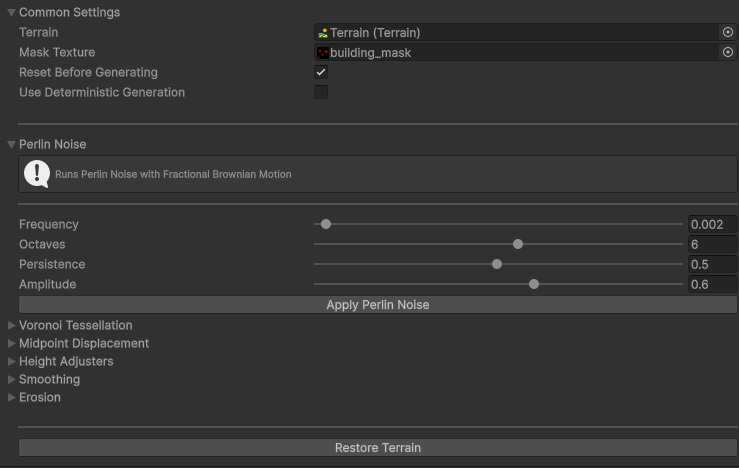
\includegraphics[width=1.0\linewidth]{img/Chapter_2_images/example_editor.png}
            \caption{The custom interface in the Unity inspector, which appears through adding the \textsf{TerrainManager} as a component to the terrain game object. We can see the mask is uploaded here, and it provides a drop-down menu for various operation. In this example, the Perlin noise parameters are shown only, as all the others have a similar layout and level of control over the operations.}
            \label{fig:manual_editor}
        \end{figure}
    \item \textbf{Evolution Window}: Dedicated interface for the Interactive Genetic Algorithm workflow, providing visual terrain variant selection and evolution controls
\end{itemize}

Both interfaces integrate with Unity's ``Extending the Editor'' \citep{UnityEditor} system and undo capabilities, allowing reversible terrain modifications during the design process.

Our system follows Unity's component-based design philosophy, with the \textsf{TerrainManager} serving as the primary component attached to Terrain objects. Additional components like \textsf{TerrainEvolutionManager} enable IGA functionality when needed.


\subsection{GPU Acceleration Implementation}
\label{Gpu_acceleration_2}

To improve performance for computationally intensive terrain operations, our system implements targeted GPU acceleration using Unity's compute shaders. GPU acceleration leverages the parallel processing capabilities of graphics hardware to perform the same operation on thousands of heightmap points simultaneously. We focus acceleration efforts on operations that usually run for multiple iterations, while maintaining robust CPU fallback mechanisms for compatibility and reliability.

\subsubsection{Architecture for GPU-Accelerated Operations}

Our GPU acceleration strategy centres on a unified \textsf{GpuTerrainOperation} base class that handles the complexities of GPU resource management, data transfer, and error handling. This architecture ensures that specific terrain operations can focus on their algorithmic logic while benefiting from consistent GPU acceleration patterns.

The base class manages several critical aspects of GPU processing:

\begin{itemize}
    \item \textbf{Resource Management}: Automatic creation and disposal of GPU textures and compute shader resources;
    \item \textbf{Data Transfer}: Efficient conversion between CPU heightmap arrays and GPU texture formats;
    \item \textbf{Error Handling}: Graceful fallback to CPU implementations when GPU processing fails;
    \item \textbf{Thread Group Organisation}: Standardised 16×16 thread group dispatch for optimal GPU utilisation.
\end{itemize}

This unified approach eliminates code duplication while ensuring consistent performance characteristics across all GPU-accelerated operations in our system.

\subsubsection{Accelerated Operations}

We implement GPU acceleration for three specific terrain operations that demonstrate high computational intensity and excellent parallelisation characteristics. While many other terrain operations could also be GPU accelerated, these three are the only ones that are typically run for multiple iterations, whereas the other operations, such as Perlin Noise, only need to run for a single iteration to achieve good results. The reason for running these three operations over multiple iterations is so that they can have an impactful and significant result on the terrain, where each iteration applies the operation to the resulting terrain of the previous iteration. 

\textbf{Enhanced Distance Smoothing}, as described in Section \ref{edbs}, represents our most sophisticated GPU-accelerated operation. This algorithm applies variable-strength smoothing based on distance from fixed points, requiring complex neighbourhood calculations and distance-aware weighting. The parallel nature of these calculations makes GPU acceleration particularly effective, as thousands of terrain points can be processed simultaneously while accessing distance information from GPU memory. 

\textbf{Basic Smoothing} implements traditional uniform height averaging, where each pixel is set to the average height of all its neighbours, with GPU acceleration. While conceptually simple, this operation benefits substantially from parallel execution when applied to large heightmaps for multiple iterations. 

\textbf{Thermal Erosion}, as described in Section \ref{thermal_erosion}, simulates material slumping through iterative height redistribution. This operation requires multiple passes over the heightmap data, making it an ideal candidate for GPU acceleration due to parallel processing of erosion calculations across all terrain points.

Each operation implements the same interface pattern, accepting heightmap data and constraint information while producing modified terrain that respects fixed height constraints.

\subsubsection{Compute Shader Implementation}

Our compute shaders follow Unity's compute shader system, utilising GPU parallel processing capabilities \cite{UnityComputeShaders}. Each shader kernel processes individual heightmap points within 16×16 thread groups, maximising GPU utilisation while maintaining memory access efficiency.

The compute shader workflow follows this pattern:

\begin{enumerate}
    \item \textbf{Heightmap Upload}: CPU heightmap data is converted to GPU format;
    \item \textbf{Constraint Mask Transfer}: Fixed point constraints are encoded as mask textures;
    \item \textbf{Parallel Processing}: Compute shader kernels process all modifiable points simultaneously;
    \item \textbf{Iterative Refinement}: Multiple passes refine results while respecting constraints;
    \item \textbf{Data Readback}: Final heightmap data is transferred back to CPU memory.
\end{enumerate}

This workflow minimizes CPU-GPU data transfer overhead by keeping data on the GPU throughout multi-iteration operations.

\subsubsection{CPU Fallback Strategy}

Since not all systems support compute shaders or have sufficient GPU capabilities, every GPU-accelerated operation in our system includes a complete CPU fallback implementation. This strategy ensures system reliability across diverse hardware configurations while maintaining identical algorithmic behaviour regardless of the execution platform.

\subsubsection{Integration with Interactive Genetic Algorithm}

GPU acceleration proves particularly valuable for the Interactive Genetic Algorithm approach detailed in Chapter \ref{Chapter4}. The IGA requires rapid generation of multiple terrain variants, making the parallel processing capabilities of GPU acceleration essential for responsive user interaction. Since each terrain operation is now quicker, running multiple of them repeatedly saves a lot of waiting time when generating different variants of the terrain.

Complete technical implementation details, including compute shader source code and resource management patterns, are available in our system's documentation and source code repository.

\section{Summary}

This chapter presented the architectural foundation of our constrained procedural terrain generation system. We identified the core requirements and design objectives that guided our approach.

We then introduced a component-based architecture that separates terrain management from specific generation algorithms, enabling flexible composition of operations through a standardised interface. 

Finally, we outlined the complete terrain workflow, from constraint identification through distance-based modification and erosion, as well as our Unity-specific implementation and GPU acceleration strategies.

This architectural foundation enables the distance-based processing methodology explored in Chapter \ref{Chapter3}. It also supports the evolutionary tuning approach presented in Chapter \ref{Chapter4}, which leverages the component system to explore complex parameter combinations through evolutionary selection.
